%Einleitungstext zum Modul
\section{Klassen}
\graphicspath{{./img/settings/}}
Alle Klassen, die für die Funktionen benötigt werden, ohne spezifische Implementierungen zu nennen.
%Bild der Klasse aus dem Klassendiagramm (nur die Klasse jeweils)
%Dokumentation zur Klasse, öffentlichen Methoden und Konstruktor sowie:
%Signal und Slots als Methoden mit Rückgabewert Sigal bzw Slot (zur kenntlichkeit)
\subsection{CAlgorithmSettingController}
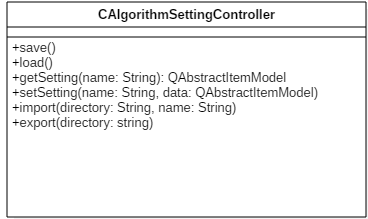
\includegraphics[scale=1, resolution=100]{CAlgorithmSettingController}\\
\beginMembers
\newMember{{save}}{void}{Speichert alle aktuellen Algorithmenparameter im Json-Format im aktuellen Arbeitsverzeichnis.}
\newMember{{load}}{void}{Lädt alle Algorithmenparameter aus dem aktuellen Arbeitsverzeichnis.}
\newMember{{getSetting}}{String name}{QAbstractItemModel}{Gibt die aktuellen Parameter des Algorithmus "name" als ItmeModel zurück.}
\newMember{{setSetting}}String name}{QAbstractItemModel data{Setzt die Parameter des Algorithmus "name" gemäß dem ItemModel "data".}
\newMember{{import}}{String directory}{String name}{Importiert die Datei "name" mit den Algorithmenparametern aus dem verzeichnis "directory".Die Datei muss im Json-Format vorliegen}
\newMember{{export}}{String directory}{Exportiert die Einstellungen aller Algorithmen in das Verzeichnis "directory".}
\closeMembers
\subsection{CGlobalSettingController}
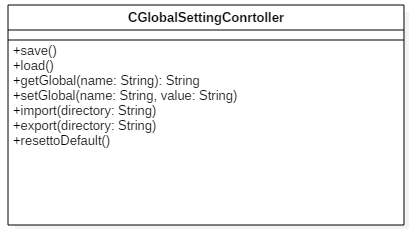
\includegraphics[scale=1, resolution=100]{CGlobalSettingController}\\
\beginMembers
\newMember{{save}}{void}{Speichert die aktuellen Globaleneinstellungen.}
\newMember{{load}}{void}{Lädt die Globaleneinstellungen.}
\newMember{{getSetting}}{String name}{String}{Gibt die Einstellung "name" als string zurück.}
\newMember{{setSetting}}String name}{String value}{Setzt den Wert "value" für die Globaleeinstellung "name".}
\newMember{{import}}{String directory}{String name}{Importiert die Datei"name" mit Globaleneinstellungen aus dem verzeichnis "directory".Die Datei muss im Json-Format vorliegen}
\newMember{{export}}{String directory}{Exportiert die Globaleneinstellungen in das Verzeichnis "directory".}
\newMember{{resettoDefault}}{void}{Stellt die Standardeinstellungen wieder her.}
\closeMembers
\subsection{QAbstractItemModel}
\includegraphics[scale=1, resolution=100]{qAbstractItemModel}\\

\subsection{CAlgorithmSettingsModel}
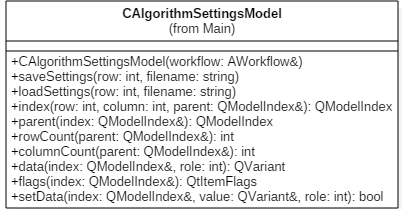
\includegraphics[scale=1, resolution=100]{CAlgorithmSettingsModel}\\
\section{Pakete}
%Einteilung der Teilmodule in Pakete 
\subsection{Paket 1}
%Bild des Pakets mit vereinfachter Klassendarstellung
%Begründung / Dokumentation / Erklärung zum Paket
\subsection{Paket 2}
%....
\section{Entwurfsmuster}
% verwendete Entwurfsmuster aufzählen erklären etc mit verinfachtem Diagramm (Klassen ohne Inhalt nur die Namen)

\section{Klassendiagramm}
\includegraphics[scale=1, resolution=100]{CSettings}\\
% Klassendiagramm des Moduls

%Bitte jeweils kleine Einleitungstexte usw in Unterkapitel gerne auch in Textform Erklärungen zufügen und auf mögliche erweiterungen durch die kann Kriterien eingehen soweit nötig !